\documentclass[11pt]{article}

\title{ECO220 Lecture Notes}
\author{Tianyu Du}
\date{\today}

\usepackage{amsmath}
\usepackage{amssymb}
\usepackage{pgfplots}
\usepackage{graphicx}
\usepackage{enumitem}
\usepackage{hyperref}
\usepackage{fancyhdr}
\usepackage{perpage}
\usepackage{float}

\lhead{Notes by T.Du}

% Lincense
\usepackage[
	type={CC},
	modifier={by-sa},
	version={3.0},
]
{doclicense}

\begin{document}
\maketitle
\doclicenseThis
\tableofcontents

\section{Lecture 1 May. 8 2018}
\paragraph{Content} Chapter 1-4,
\begin{itemize}
	\item Statistics
	\item Data
	\item Population
	\item Sample
\end{itemize}

\subsection{Statistics}
\paragraph{What is statistics} Quantitive methods.
\subsubsection{Example 1}
	\paragraph{Question} This summer, 120 students enrolled in ECO220. Find out the number of courses that students are taking, the average number of courses they take, and the $\%$ of student taking 1 or 2 courses.

	\paragraph{Population} 120 students in ECO220. Noted as $N = 120$
	
	\paragraph{Analyze:}
	\begin{enumerate}
		\item Number of courses they take.
		\item Average number of courses they take.
		\item Percent of students taking 1 or 2 courses.
	\end{enumerate}
	
	\paragraph{Data} information collected from the whole \emph{population} (all individuals). Use data to answer questions above.
	
	\begin{center}
		\begin{tabular}{|c|c|c|}
			\hline
			number of courses & number of students & percent \\
			\hline \hline
			1 & 40 & 0.33 \\
			\hline
			2 & 30 & 0.25 \\
			\hline
			3 & 30 & 0.25 \\
			\hline
			4 & 15 & 0.14 \\
			\hline
			5 & 5 & 0.03 \\
			\hline
			Total & 120 & 1.00 \\
			\hline
		\end{tabular}	
	\end{center}
	
	\begin{figure*}[h]
		\centering
		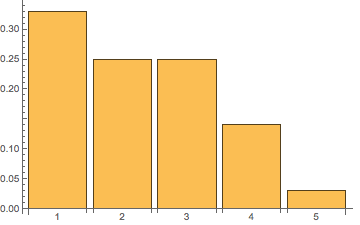
\includegraphics[width=0.7\linewidth]{eco220pic/fig1}
		\caption{Frequency}
	\end{figure*}
	
	\paragraph{Parameters} Parameters are fixed numbers. They can be calculated once we measure everyone in population.
	\newline
	\underbar{Examples of parameters from population} 
	\begin{itemize}
		\item \textbf{Average} $\mu = 2.29$
	\end{itemize}

\subsubsection{Example 2} 
	\paragraph{Question} Find out the percentage of people in Ontario who are in favour of government policy.
	
	\paragraph{Population} People in Ontario.
	\begin{center}
		\begin{tabular}{|c|c|c|}
			\hline 
			In favour of policy & \# of people in Ontario & \% \\
			\hline \hline
			Very much in favour & * & * \\
			In favour & * & * \\
			neutral & * & * \\
			not in favour & * & * \\
			strongly against & * & * \\
			\hline
			Total & $N$ = Population of Ontario & 1.00 \\
			\hline
		\end{tabular}
	\end{center}
	\paragraph{Sample} Since $N$ is too large to handle, we select a sample, which is a subset of population, denoted as $n$, and then analyze the sample.
	
	\begin{center}
		\begin{tabular}{|c|c|c|}
			\hline 
			In favour of policy & \# of people in Ontario & \% \\
			\hline \hline
			Very much in favour & & \\
			In favour & &\\
			neutral & & \\
			not in favour & & \\
			strongly against & & \\
			\hline
			Total & $n$ = Size of sample & 1.00 \\
			\hline
		\end{tabular}
	\end{center}
	\paragraph{} The above chart based on sample data to \emph{estimate} the chart using population data. 
	
	Let $p$ be the \% of people in Ontario(population) who are "very in favour" or "in favour"
	
	Let $\hat{p}$ be the \% of people in sample who are "very in favour" or "in favour", can be calculated based on the sample data.
	
	\paragraph{}The parameter $p$ has an unknown value. The value of $\hat{p}$ can be calculated from sample data, $\hat{p}$ is an \textbf{estimate} for $p$.
	
	\paragraph{Note} $p$ is a fixed value, but $\hat{p}$ will change from sample to sample. We call $\hat{p}$ an \textbf{estimator} (or \textbf{sample statistic}). The value of sample statistic will change from sample to sample, we call $\hat{p}$ a \emph{random value}.
	\newline \quad
	\newline
	\textbf{Parameters} on population
	\begin{itemize}
		\item $\mu$: Average
		\item $p$: Percentage
	\end{itemize}
	\textbf{Sample Statistic} on sample
	\begin{itemize}
		\item $\overline{x}$: Average
		\item $\hat{p}$: Percentage
	\end{itemize}
	\paragraph{Statistics}
	\[
	\text{Statistics}
		\begin{cases}
			\text{Descriptive statistics}
				\begin{cases}
					\text{Graph} \\
					\text{Numerical measures} \\
				\end{cases}
			\\
			\text{Inferential statistics: \emph{Draw conclusions on a population based on sample data.}} \\
		\end{cases}
	\]
	
	\section{Lecture 2 May. 9 2018}
	\paragraph{} What is statistics? \textbf{Population} with size denoted with $N$ and \textbf{sample} with its size denoted as $n$. Analyze the population from data from sample.
	
	\subsection{Inferential statistics} Involves \emph{uncertainty}, to deal with the uncertainty, we need \textbf{probability}
	
	\subsection{Data}
	\paragraph{}Two types of data
	\begin{enumerate}
		\item Quantitive data
			\begin{enumerate}
				\item Discrete
				\item Continuous
			\end{enumerate}
		\item Qualitative(Categorical) data 
	\end{enumerate}
	\paragraph{Note} Some categorical data might be sensitive (e.g. income, age), to handle this, we could \textbf{categorize} the answers to handle this while collecting data.
	
	\subsection{Descriptive Statistics: Graphs}
	\paragraph{Example 1} Incomes in Toronto.
	\paragraph{Example 2} Market shares of computers.
	\paragraph{Example 3} Home price in Toronto.
	\paragraph{Example 4} Age and income
	
	\paragraph{Note} There is no unique (or, correct) way of drawing graphs. A good graph is a picture that tells the audience a true picture of a population or sample.
	
	\subsection{Descriptive Statistic: Numerical Measures}
	\subsubsection{Measures of centre (location)}
	\paragraph{Mean} also called average and expected value, let $x_1, x_2, \dots x_n$ be the measurements for the population of size $N$. The \underbar{population mean} is denoted by $\mu$ and defined as 
	\[
		\mu = \frac{1}{N} \sum_{i=1}^N x_i
	\] Let $x_1, x_2, \dots, x_n$ be measurements for the sample of size $n$, then the \underbar{sample mean} is denoted by $\overline{x}$ and defined as
	\[
		\overline{x} = \frac{1}{n} \sum_{i=1}^n x_i
	\]
	
	\textbf{Note} $\mu$ is population mean, therefore a \emph{parameter}. That's $\mu$ has a \emph{fixed value} if all units in population is measured. $\overline{x}$ is sample mean, and therefore a \emph{sample statistic (estimator)} and $\overline{x}$ does not have a fixed value. The values of $\overline{x}$ change from sample to sample.
	
	\textbf{Note} The mean is a good measure of centre, but it is sensitive to extreme values.
	
	\paragraph{Median} is the value in the middle when all data are sorted in order of magnitude.
	
	\textbf{Note} For the data set with event numbers of observations, we defined the median as the mean of values of two observations in the middle.
	
	\textbf{Note} 50\% of data are less than the median.
	
	\paragraph{Mode} the value(s) that occurs most often.
	
	\textbf{Note} there could be multiple modes in a dataset. (if there are tow modes, the data is called \textbf{bimoded}). Also it is possible for a dataset to have \textbf{no mode}(e.g. values of all observations are unique).
\end{document}














